\chapter{Semi Automatic Annotation} \label{chapter:semi_automatic}

To assist the process of manual image annotation presented in chapter \ref{chapter:image_pose_annotation}, a neural network is to be developed to suggest poses. A neural network requires proper configuration and expertise to train it. This chapter describes the network architecture and its variations, as well as different approaches to train the network and the modified annotation process resulting from the usage of the network.

\section{Terminology}

\noindent\textbf{Residual Connections.} A \textit{residual connection} (or skip connections) is a part of a neural network that skips some nodes of the network and adds the input directly to a deeper layer of the network. They can prevent the problem of the gradients becoming very small in very deep networks, which prevents proper updating of the weights. Fig. \ref{fig:residual_connection} visualizes such a connection. \\

\noindent\textbf{Depth Image.} A \textit{depth image} is an image $D$ that contains the distance $d$ of the camera to the surface for each pixel $u$ in an image $I$. Depth images can be created using special cameras or from stereo images and are often used in pose estimation and other computer vision tasks.

\section{Network Architecture}

\begin{figure}[!tbp]
	\centering
    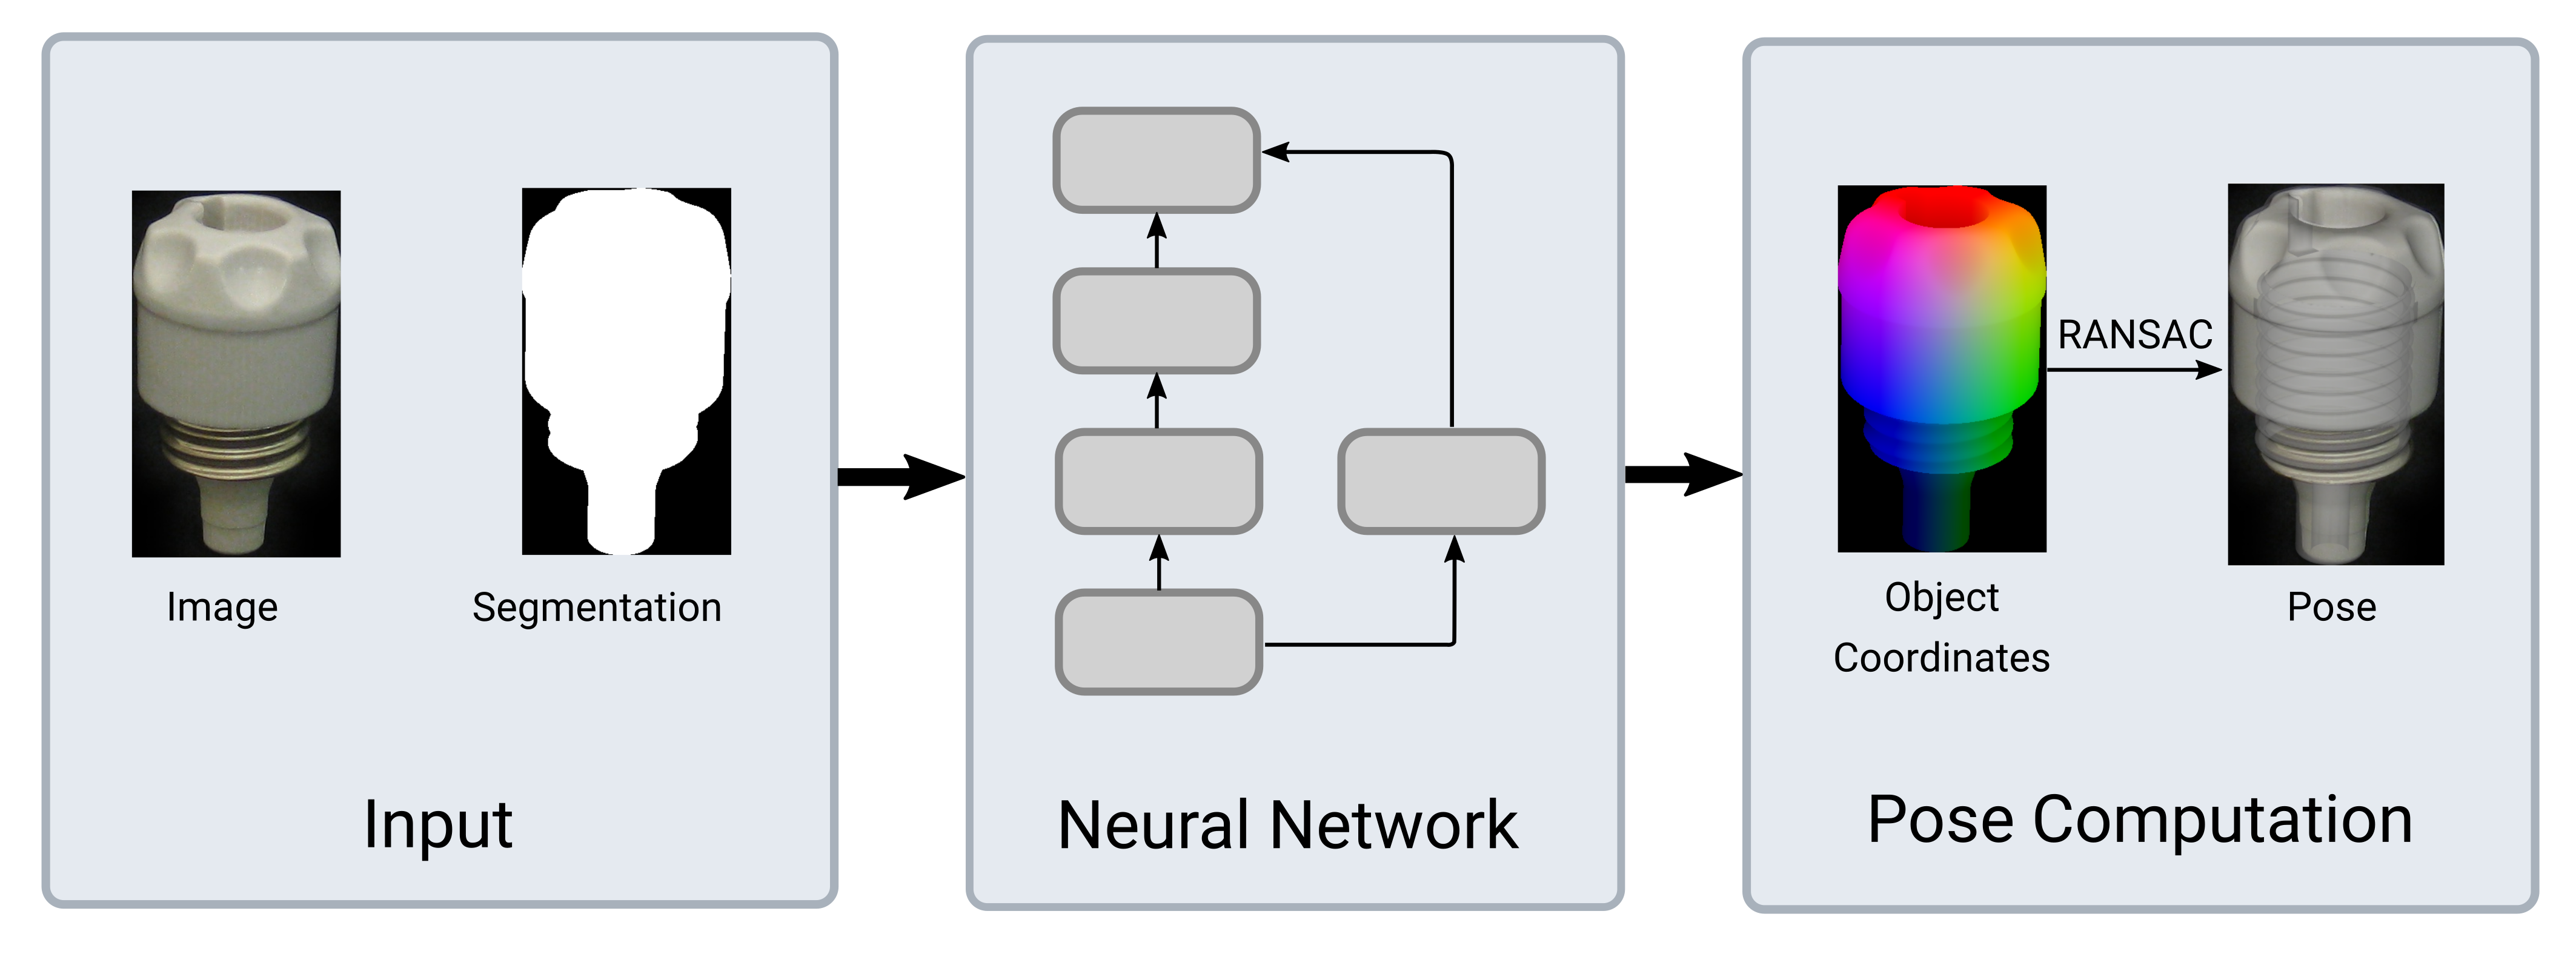
\includegraphics[width=\linewidth]{network_pipeline}
    \caption{The schematic pipeline of the neural network. The input to the network are the image and the corresponding segmentation image. The neural network then uses the segmentation to retrieve the pixels to predict object coordinates for. In the final pose computation stage the object coordinates and their 2D locations are used to retrieve the best pose using RANSAC. The object's transparency has been decreased to render the final pose. Own image.}
    	\label{fig:network_pipeline}
\end{figure} 

The architecture of the network is adapted to the problem specific to the medical images. This means that the network expects segmentation masks to be present. There is no mechanism of inferring the masks. This reduces the the 6D problem significantly the complexity of predicting the position of the object. Contradicting object coordinates output by the network can still lead to incorrect poses though. This precondition lead to the pipeline visible in fig \ref{fig:network_pipeline} which takes the actual image and the segmentation image as input. The images shown are cropped already to the segmentation mask but in later applications the image size and proportion of pixels belonging to the object can be arbitrary. It is important to note, that the network does not take depth images as input opposed to many other pose estimation approaches. This is owed to the nature of the provided medical images which do not contain depth information.

The architecture that is chosen as the basis for the network itself is called ResNet. ResNet was first presented in \cite{resnet} and enabled researchers to create deeper networks than before. The vanishing gradients problem describes the phenomenon that the gradients gradually become 0 during backpropagation in very deep networks. This can be partly compensated by re-adding the inputs of earlier layers to the output of later layers. A residual connections can be seen in fig. \ref{fig:residual_connection}. Fig. \ref{fig:resnet_comparison} shows a comparison with the wide-spread and well known architecture \textit{VGG} \cite{vgg}.

To obtain an optimal architecture multiple variations of the basic structure that can be seen in fig. \ref{fig:network_architecture} are created. The deeper version consist of more repetitions of the inner blocks. For comparison reasons two models are created that replace the batch normalization layers with dropout layers.

\begin{figure}[!tbp]
	\centering
	\begin{subfigure}[t]{0.47\textwidth}
		\centering
    	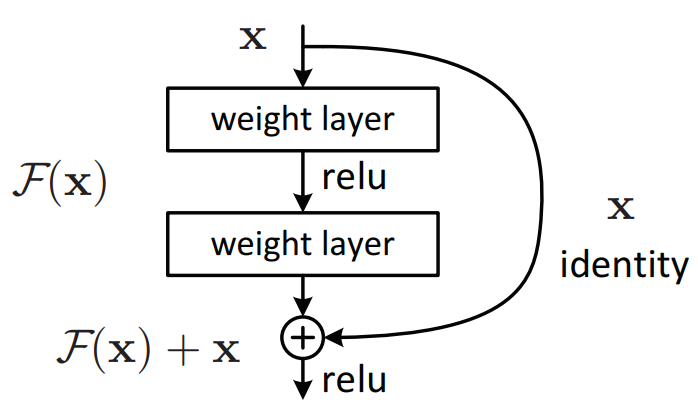
\includegraphics[width=\linewidth]{residual_connection}
    	\caption{A detailed view on a residual connection. The residual connections add the input of earlier layers of the network to deeper ones.}
    	\label{fig:residual_connection}
	\end{subfigure}
	\hfill
	\begin{subfigure}[t]{0.47\textwidth}
		\centering
    	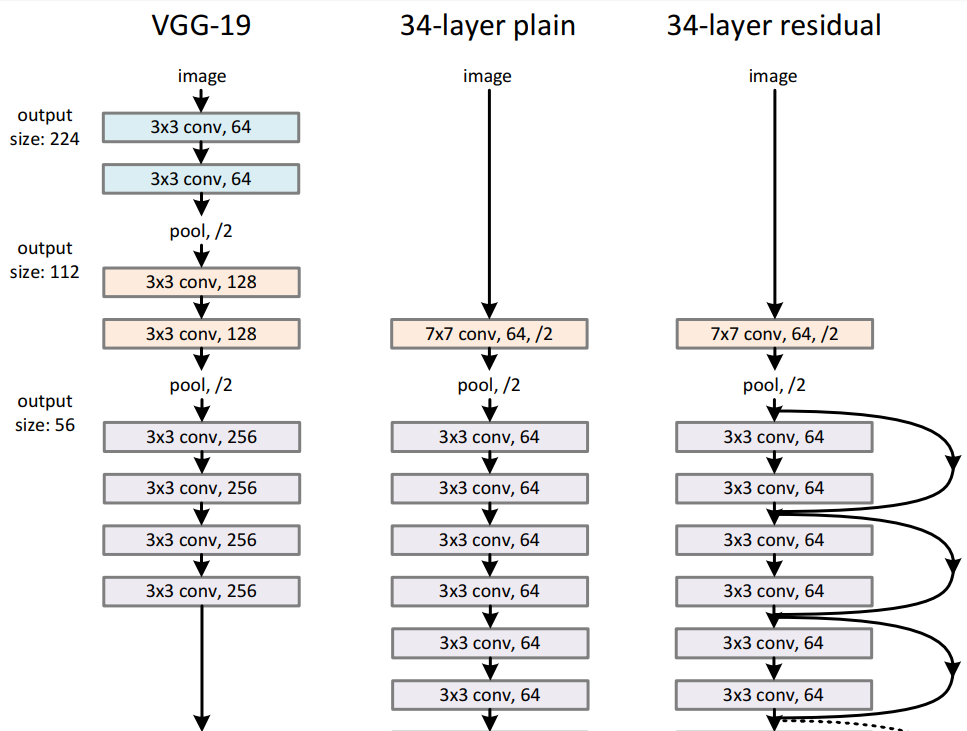
\includegraphics[width=\linewidth]{resnet_comparison}
    	\caption{Excerpt of a comparison between the ResNet architecture and VGG. The ResNet allows the creation of deeper network as the problem of vanishing gradients, i.e. very small gradients at deeper layers, can be targeted this way. The image has been cropped.}
    	\label{fig:resnet_comparison}
	\end{subfigure}
	\caption{A key component of ResNet: the residual connection. Left shows the connection in detail and right shows a comparison with the VGG architecture. Images from \cite{resnet}.}
	\label{fig:resnet_details}
\end{figure} 

\begin{figure}[!tbp]
\end{figure} 

\begin{figure}[!tbp]
	\centering
    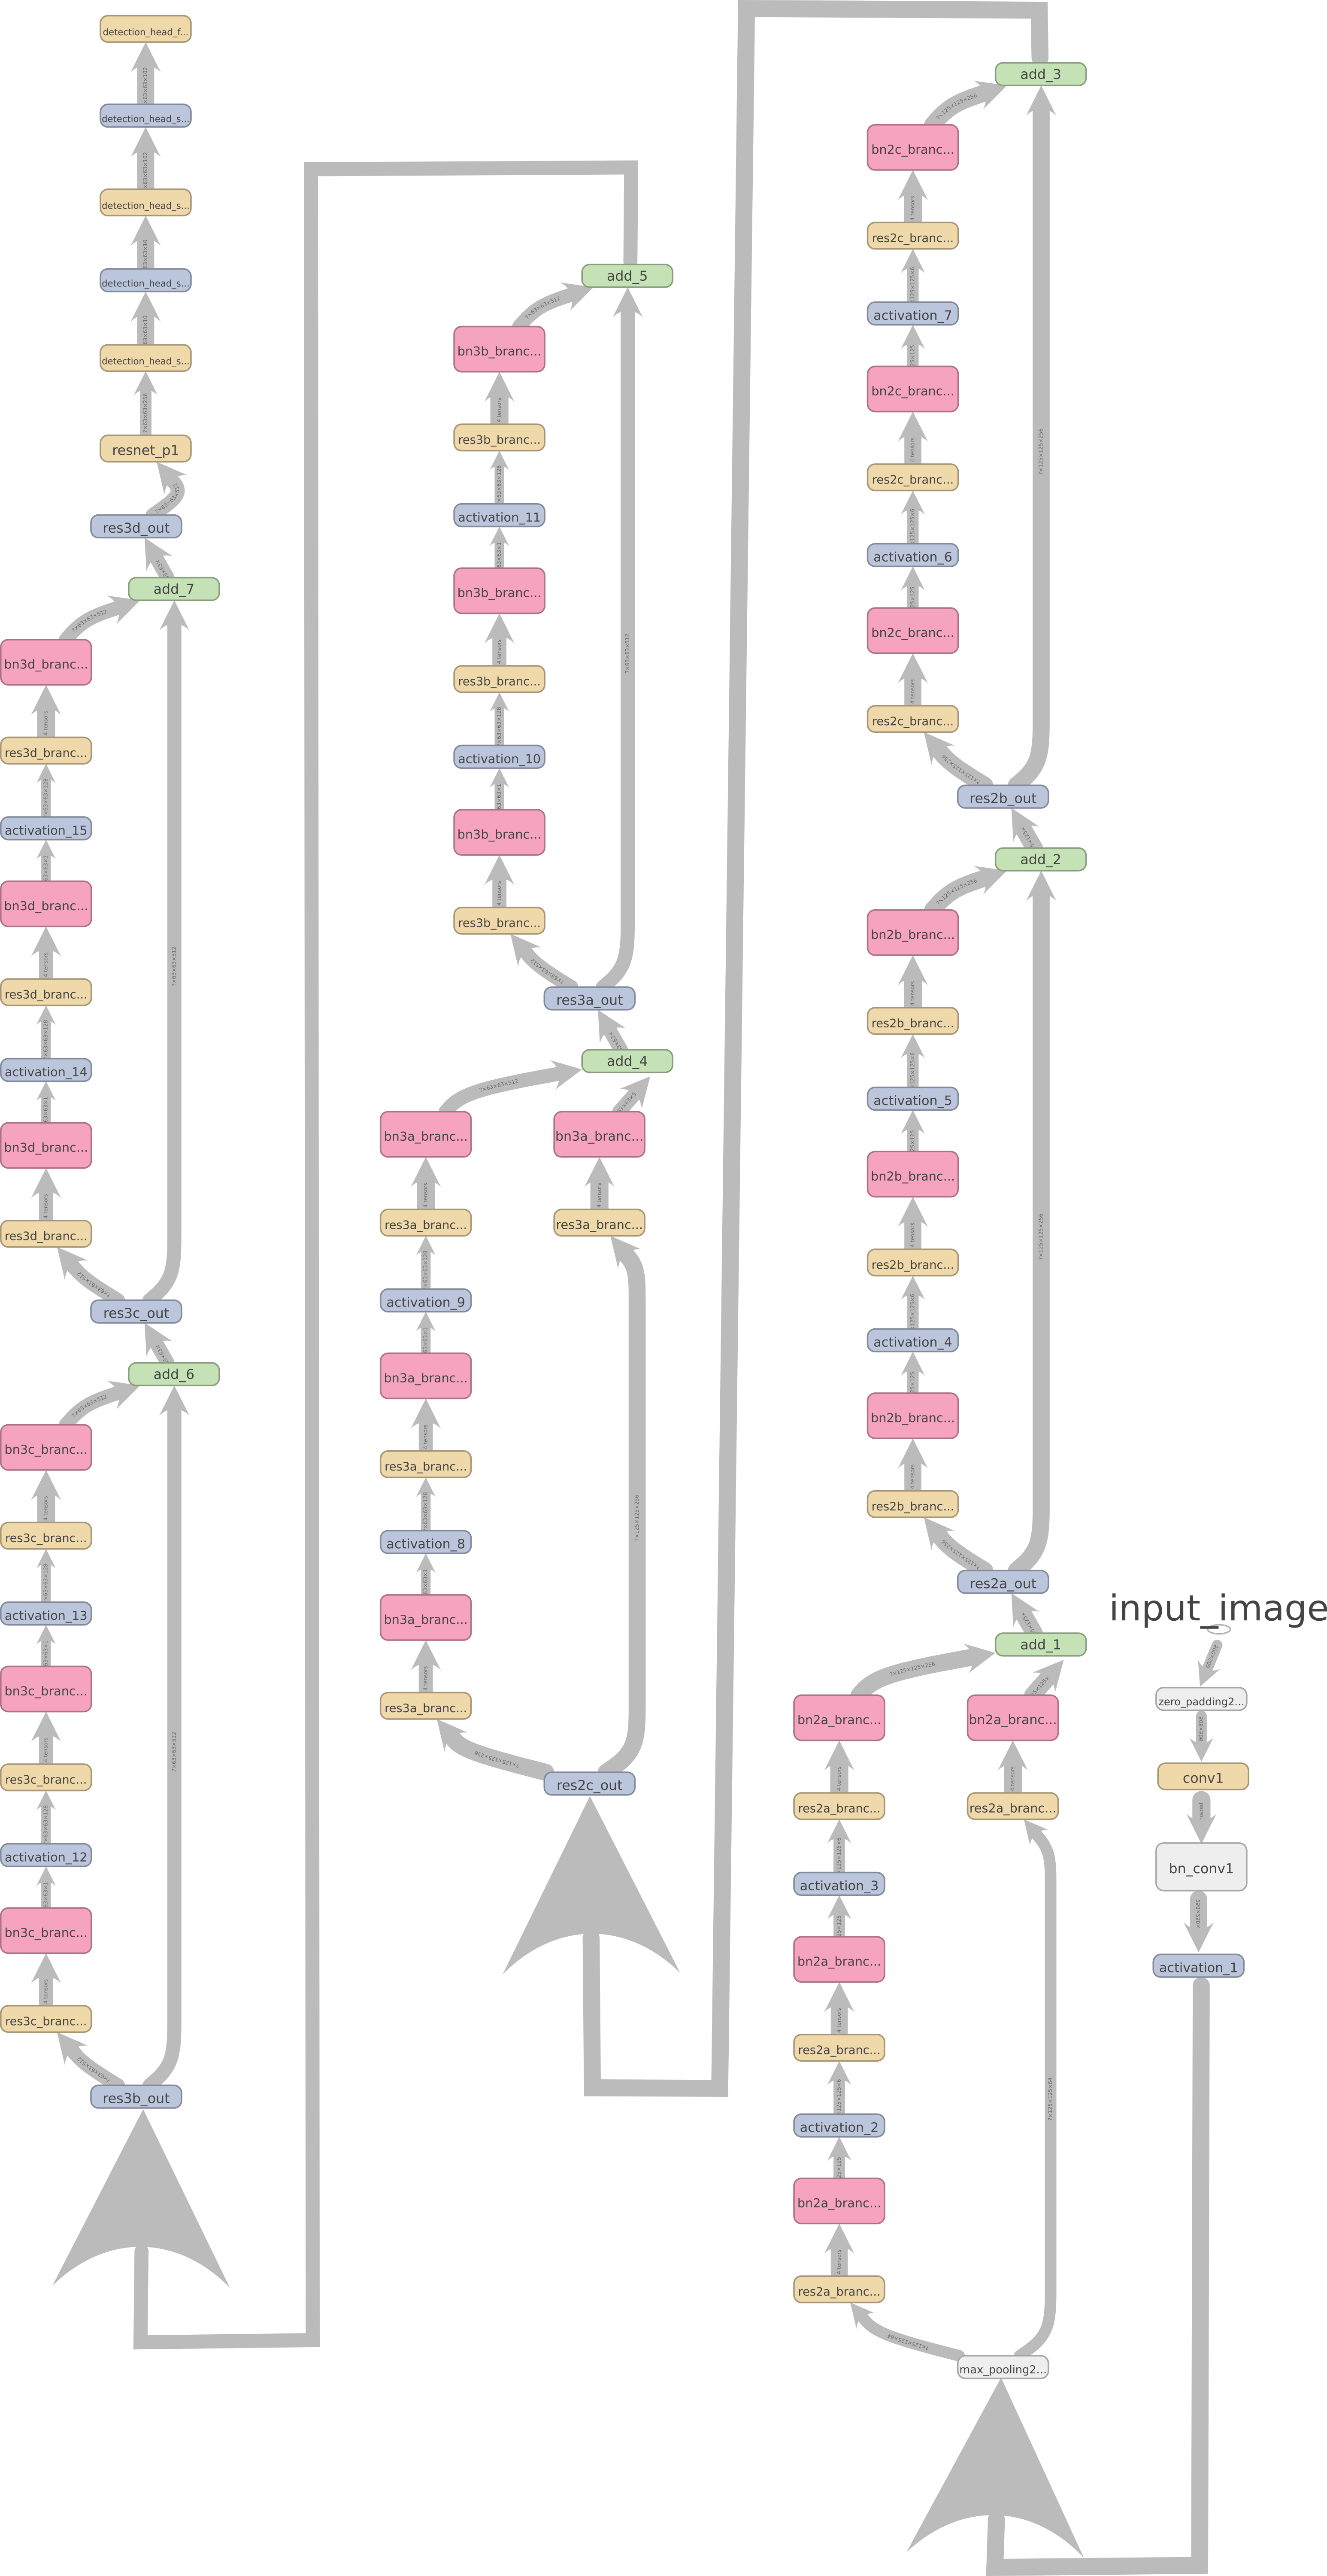
\includegraphics[width=0.75\linewidth]{network_architecture}
    \caption{An overview of the shallower architecture used in the project. The visualization was created using \textit{Tensorboard} but modified to fit one page. The large arrows have no meaning and are only there to emphasize where the network continues. Own image.}
    	\label{fig:network_architecture}
\end{figure}

\section{Methods}

% Describe the whole workflow of annotating images using the program
% and then training the network / predicting poses

% Describe the two different approachs of training the network

\subsection{Training from Scratch}

\subsection{Incremental Training}

\subsection{Inference}

% Manual inference for large batches

% Inference in the program